\section{Factores productivos}
\textbf{Nos preguntamos:} ¿Qué pasa cuando lso empresarios quieren maximizar los factores productivos? \emph{Respuesta: Cuando alguien no aporta mucho valor a la sociedad se produce una ``Japonisación'' de la sociedad, hoy en día los salarios mínimos de Japón causaron que estén retrasados casi ya tres décadas.} \textbf{Ejemplo: } El ejemplo del cafe, la productividad por trabajador incrementa nos es la suma de sus partes, siempre se produce más, un barista mas otra no producen el doble, producen más que el doble. \newline 

\subsection{La productividad de los trabajadores}
En la economía la curva tiene la forma de campana, hay una cantidad de trabajadores que son el nivel ótpimo
\begin{figure}[htbp]
    \centering
    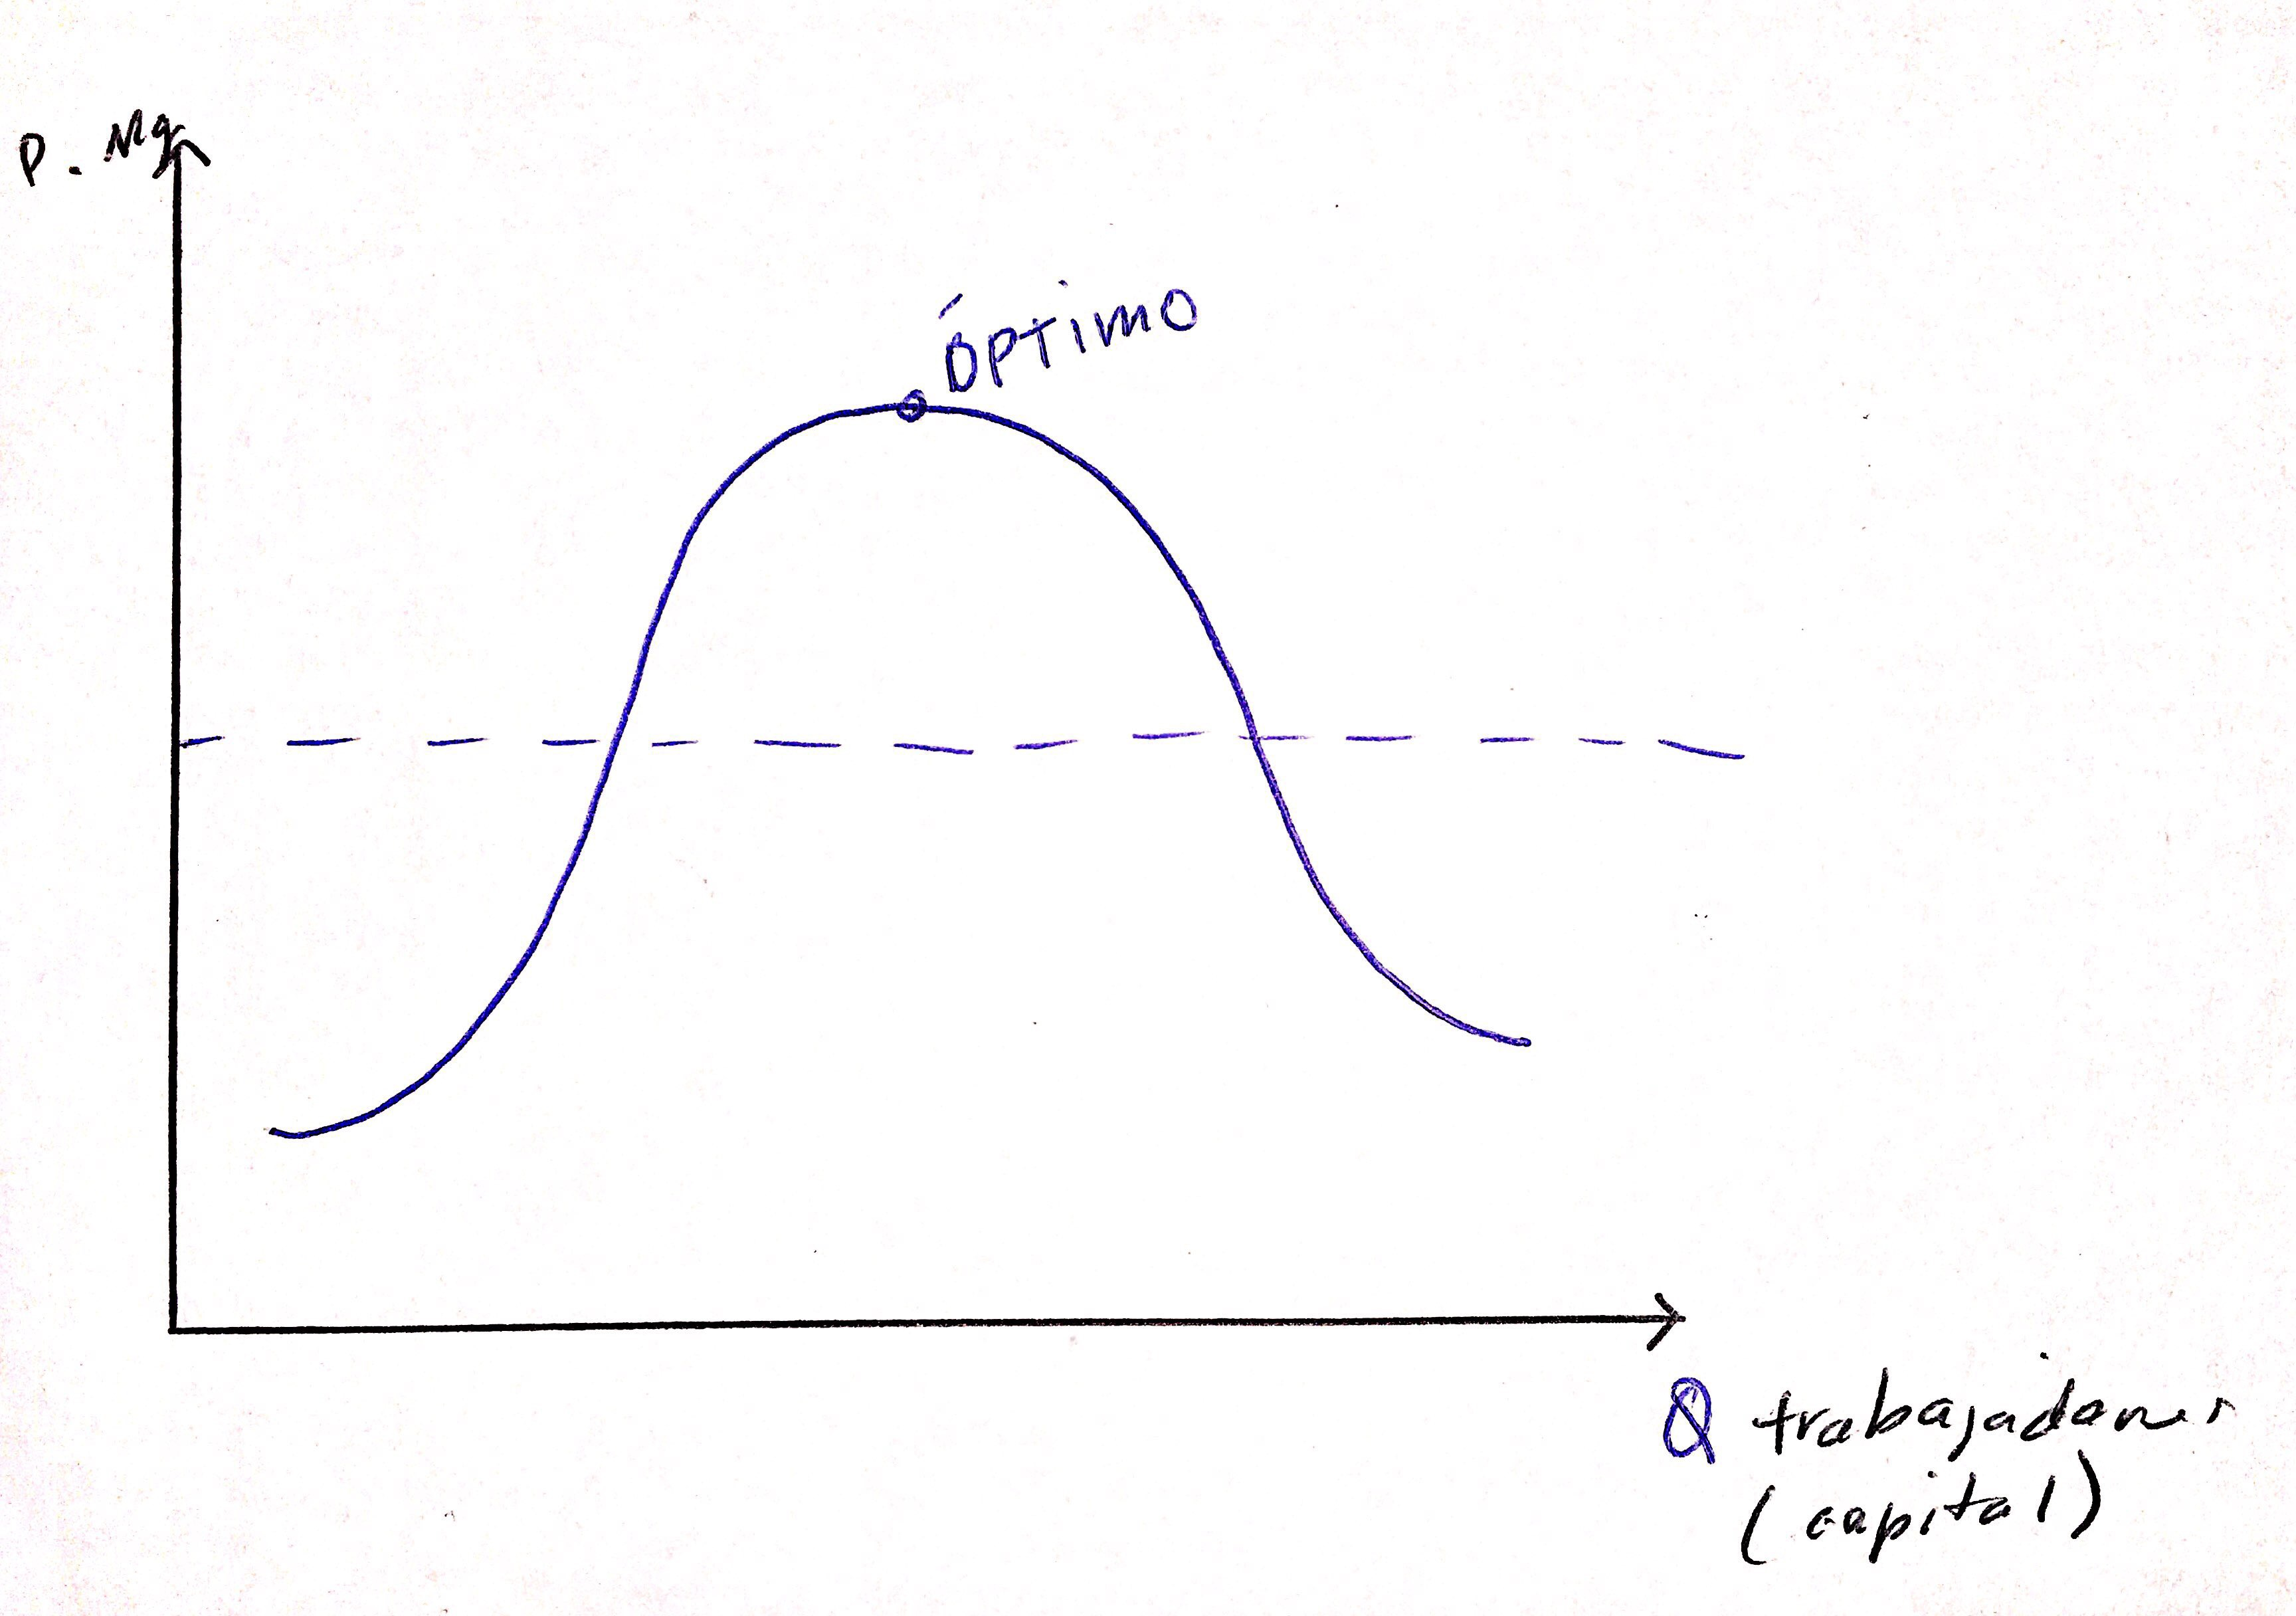
\includegraphics[width=10cm]{Classes/Images/2019-07-31-1}
    \caption{porductividad de lso trabajadores, dos recursos (la productividad marginal y la cantidad de trabajadores(capital))}
    \label{}
\end{figure} 

\[
  A_{\text{cafés 5 empleados}} = 50 \frac{\text{unidades}}{\text{hora}}\qquad P_{empleados} = 10 \qquad\Rightarrow  10*(20) = Q200
\]
\[
  Q_{\text{café 6 empleados}} = 33 \frac{\text{unidades}}{\text{hora}}  \qquad P_{empleados} = 9.17/h \qquad \Rightarrow  9.17*(20) = Q183.4
\]
\[
  Q_{\text{cafe 7 empleados}} = 52 \frac{\text{unidades}}{\text{hora}}\qquad P_{empleados} = 7.42/h \qquad \Rightarrow  7.42*(20) = Q148.57
\]s


\section{Tema de hoy}
El conocimiento de la función empresarial es práctico no articulable, es el conocimiento que se adquiere cuando un niño aprende a montar la bicicleta. \newline 
\textbf{Crimen y castigo, recomendado} \emph{\textbf{Paréntesis:} hace un cálculo, la sociedad que matan y roban desaparecen, \textbf{Ejemplo: } el imperio ottomano.} Las sociedades que tienen mejores reglas son las que más transcienden. \newline 
El derecho es un conocimiento tácido, en el derecho romano las reglas no se justificaban o evadían por ignorancia, \emph{\textbf{Respuesta:}la mayoría de gente no sabe por qué robar está mal solo lo sabe por que es un concoimiento tácido no articulable.}

\subsection{El carácter creativo de la función empresarial}
Para ser empresario no se necesita nada más que una idea, ya teniendo una buena idea el capital aparece. Los empresarios se dan cuenta de la descoordinación en el mercado, \textbf{Ejemplo: } el arbitraje o especulación. Beneficios empresariales puros son los que surgen derivados de solucionar situaciones de descoordinación. \newline 
En el ``stick analisis'' se demuestra en el potencial de la función empresarial, \textbf{Ejemplo: } la maldición de Tejas \emph{Paréntesis:El petrolio era una maldición ya que las vacas se tragaban el petrolio y la gente odiaba el petroleo, hay lugares que la basura para ellos es oro para nosotros, la gente está descoordinada, la coordinación de produce a partir de la función empresarial.} Por consiguiente la persona que consideraba su basura sin valor, a raíz de la coordinación, empieza a apreciar lo que consideraba basura. \newline 
Los monopolios se producen cuando no hay competencia, la persona que tiene una excelente idea que se mete a la política buscando implementar su idea bajo la ala de 0 competencia es una persona mierda.
\newline 
Esta implementación de ideas que producen coordinación y el arbitraje muy conveniente no dura mucho ya que otros imitan esta idea y coordinan hasta equilibrar el precio. Poco a poco no se vuelve rentable.




\subsection{coordinación y ajuste}
El ranchero que tiene petrolio ajusta su comportamiento a necesidades de terceros(ultimo usuario) por que está en mi interés, y el usuario final entiende que en efecto sí hay recurso y dispone otros bienes para comprarlos, el refrán de el agua de mayo, la persona A y B están de espaldas, el empresario les da vuelta. Este es e proceso de mercado. Hasta el empresario mas subido se hace rico plegando a las necesidades de los demás.

\subsection{Efectos del beneficio empresarial}
\emph{\textbf{Paréntesis:}Los intelectuales usualmente son los que más oponen la libre empresa, por resentimiento y envidia. El proceso social no entiende esto.} \newline 
\newline 
Ganancia: una señal muy poderosa para los empreesarios 
\newline 

\emph{Citación:``A donde no puedo apropiarme de los frutos de mi trabajo desaparece la función empresarial"} \newline 
Lo que está en nuestro interés nos incentiva a buscar información, por eso en los casos de descoordinación en el mercado es el empresario el que ejerce la función empresarial. \newline 
\emph{\textbf{Paréntesis:}} en las drogas legales hay avances e innovaciones, pero en las illegales no está en los interéses de las personas que venden cocaína por ejemplo innovar su droga.
\textbf{Ejemplo: } The SilkRoad (empresa de venta de drogas), era el amazon de las drogas illegales, se transmitía la info que le interesaba a los consumidores. La persona que generá la plataforma de SilkRoad coordinó a todo el mercado de drogas.



\subsection{Ayuda social}
El incentivo se diluye en la ayuda social, quita el incentivo de buscar la información para coordinar a la sociedad cae. ``Ayudar a la gente'', impide su desarrollo y quita a los empresarios que si resuelven descoordinaciones.
\emph{\textbf{Paréntesis:} Numero de damba, 150 la capacidad de el ser humano de formar relaciones son de 150}. Significa que durante miles de años hemos estados en grupos trivales compuestos de 150 personas, el cableado interno es que funciona bien ya que todo funciona mejor en sociedades pequeñas. El altruismo y solidaridad funciona en pequeños grupos.
\newline 
Los porblemas de redistribución de la renta.
